In Contrastive Multi-view Coding (CMC) \cite{tian2020contrastive} the authors start from the framework proposed in CPC, but they adapt it to maximize the mutual information between different views of the same image, removing the prediction part and focusing on contrastive learning. Suppose we have two different views of a dataset $V_1$ and $V_2$, and we build a dataset that consist of a collection of samples $\{v_1^i, v_2^i\}_{i=1}^N$. We consider positive pairs those which are sampled from the joint distribution $x \sim p(v_1, v_2)$ where $x= \{v_1^i, v_2^i\}$, while we consider negative samples those sampled from the product of marginals $y \sim p(v_1)p(v_2)$ where $y = \{v_1^i, v_2^j\}$. The goal is to learn a critic function $h_\theta$ which is trained to output high values for positive pairs and low values for negative pairs. In this way we can use a contrastive loss function that we can use to train the model to correctly select a single positive sample out of a set that contains $k$ negative samples:
\[\mathcal{L}^{V_1, V_2}_{contrast} = -\mathbb{E}_{\{v_1^1, v_2^1, \dots, v_2^{k+1}\}} \Bigg[ \log \frac{h_\theta(\{v_1^1, v_2^1 \})}{\sum_{j=1}^{k+1}h_\theta(\{v_1^1, v_2^j \})}  \Bigg] \]
where $\{v_1^1, v_2^1 \}$ is the positive pair and $\{v_1^1, v_2^j \}$ with $j > 1$ is the a negative pair. To extract the latent representations of $v_1$ and $v_2$ we use two encoders $f_{\theta_1}(\cdot)$ and $f_{\theta_2}(\cdot)$. We compute the latent representations $z_1 = f_{\theta_1}(v_1)$ and $z_2 = f_{\theta_1}(v_2)$ which we can use to compute the output of the critic as:
\[ h_\theta(\{v_1, v_2\}) = \text{exp}\Bigg(\frac{z_1^Tz_2}{\lVert z_1\rVert \lVert z_2\rVert}\cdot \frac{1}{\tau}\Bigg) \]
In the formulation of $\mathcal{L}^{V_1, V_2}_{contrast}$ the view $V_1$ is used as anchor view, while we enumerate samples from view $V_2$, but we can also do the opposite and use the following loss:
\[ \mathcal{L}(V_1, V_2) = \mathcal{L}^{V_1, V_2}_{contrast} + \mathcal{L}^{V_2, V_1}_{contrast} \]
After the training phase, if we want for instance to fine-tune the model on an image classification task, we can concatenate the output of the two encoder networks $f_{\theta_1}$ and $f_{\theta_2}$ and use it as input of a classification network.
In the paper the authors prove that the optimal critic $h^*_\theta$ is proportional to the density ratio between the joint distribution $p(z_1, z_2)$ and the product of the marginals $p(z_1)p(z_2)$:
\[ h^*_\theta(\{ v_1,v_2\}) \propto \frac{p(z_1, z_2)}{p(z_1)p(z_2)} \propto \frac{p(z_1|z_2)}{p(z_1)} \]
that is the point-wise mutual information and from this the same bound obtained for CPC can be derived:
\[I(z_i;z_j) \ge \log(k) - \mathcal{L}_{contrast} \]
hence minimizing the contrastive loss yields to the maximization of the mutual information between the latent representation of the different views.\\
Then the authors proposes two different ways for extending the this framework to the usage of multiple views. Suppose we have $M$ different views of a dataset $V_1, \dots, V_M$, we can extend CMC to the multiple views case using the following losses:
\[ \mathcal{L}_C = \sum_{j=2}^{M} \mathcal{L}(V_1, V_j), \qquad \mathcal{L}_F = \sum_{j=1}^{M} \sum_{i=1}^{j-1} \mathcal{L}(V_i, V_j)\]
in the core view formulation ($\mathcal{L}_C$) we select one view that we want to optimize, for instance $V_1$, and we build a pairwise representations between $V_1$ and all the other views. In the full graph formulation ($\mathcal{L}_F$) we instead consider all the possible pairs. The full graph formulation is more computational expensive but it has the advantage that it allows to capture more information between different views.\\
In order to achieve good results using many negative examples in the contrastive loss, CMC uses a memory bank to store latent representations for each training sample, so that a certain amount of negative samples can be retrieved from the memory bank without recomputing the features each time. The drawback of course is the fact the representations in the memory becomes old after some time and they must be updated after some time.\\
In the experiments in order to produce different views of the images, they convert the images from the RGB to the Lab representation, and then they split each image into L and ab channels. Of course L and ab from the same image are considered positive pairs. They do the same thing for the YDbDr color space, splitting the Y and DbDr channels. For testing the multi-views case they again use the Lab representation separating the L and ab channels, and they also include other three views depth, surface normal and semantic labels (example in figure \ref{fig:cmc-views}).
\begin{figure}[H]
	\centering
	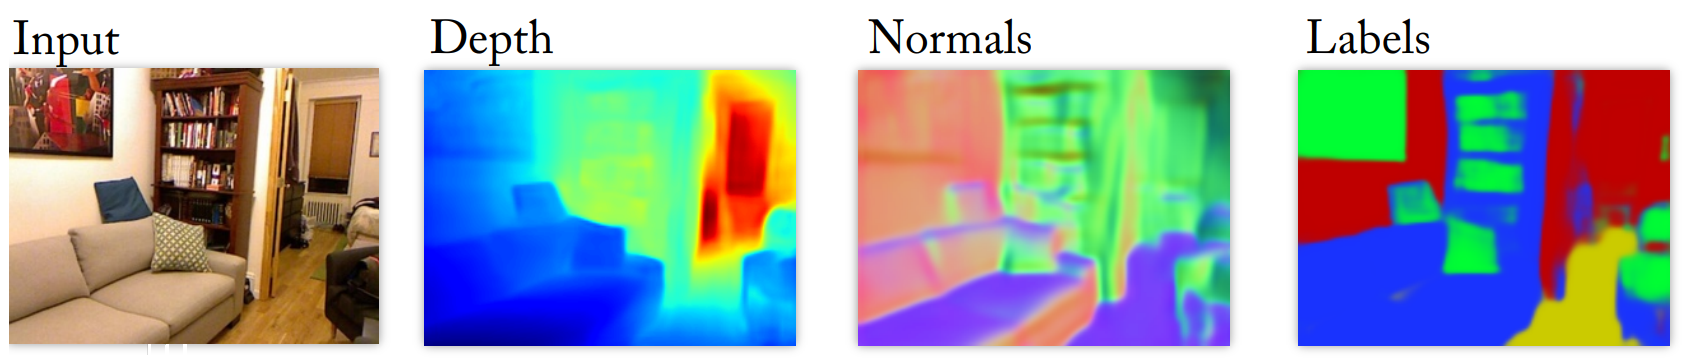
\includegraphics[width=10cm]{./images/cmc-views.png}
	\caption{Example of depth, normal and semantic labels views of an image}
	\label{fig:cmc-views}
\end{figure}
